\documentclass[ascpectratio=169]{beamer}

\usepackage{graphicx}
\usepackage{outlines}
\usepackage{multicol}

\usetheme{PaloAlto}
\usecolortheme{whale}

\addtobeamertemplate{footline}
{%
  \usebeamercolor[fg]{title in sidebar}
  \vskip-1cm\hskip10pt
  \insertframenumber\,/\,\inserttotalframenumber\kern1em\vskip2pt%
}

\title{Nuclear War City Simulator 2019 Xtreme Edition}
\author[]{Josef Bostik \\
  Thomas van Haastrecht \\
  Eric Pereira \\
  Ryan Wojtyla}
\date{March 15, 2019}

\begin{document}

%----------BEGIN TITLE----------

\begin{frame}
  \titlepage
\end{frame}

%-----------END TITLE-----------

\section{Origins}

%----------BEGIN ORIGINS----------

\begin{frame}

  \frametitle{Initial Ruminations}

  \begin{center}
    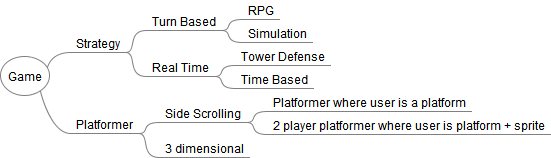
\includegraphics[scale=0.5]{../../Diagrams/Game/Game.png}
  \end{center}

\end{frame}

%-----------END ORIGINS-----------

%----------BEGIN KIND OF GAME----------

\begin{frame}

  \frametitle{Settlement}

  \begin{multicols}{2}
    
  \begin{outline}
    \1 turn-based strategy
    \1 2D grid
    \1 rogue-like
      \2 short
      \2 procedurally generated (we hope)
      \2 high replayability
  \end{outline}

  \columnbreak


  \end{multicols}

\end{frame}

%-----------END KIND OF GAME-----------

\section{Game Engine}

%----------BEGIN GAME ENGINE----------

\begin{frame}

  \frametitle{Game Engine}


\end{frame}

%-----------END GAME ENGINE-----------

%----------BEGIN USING GODOT----------

\begin{frame}

  \frametitle{Working with Godot}

  \begin{outline}
    \1 Steep initial learning curve
    \1 Official Godot documentation is expansive, but it lacks examples.
    \1 Community tutorials are more example-based.
    \1 Recent updates have obsolesced a significant portion of provided
    community support.
      \2 solutions for the old system
  \end{outline}

  \vspace*{1cm}

  \begin{outline}
    \1 The learning curve soon plateaus.
    \1 The native scripting language, GDScript, is nice to use.
    \1 An extensive collection of objects is provided.
  \end{outline}

\end{frame}

%-----------END USING GODOT-----------


\section{Foundations}

%----------BEGIN PREMISE----------

\begin{frame}

  \frametitle{Story}

  \begin{center}
    {\Large Prepare for imminent global thermonuclear war!}
  \end{center}

  \begin{outline}
    \1 Ensure the survival of as many of your citizens as possible.
    \1 Pacify the masses.
    \1 Manage resources.
    \1 Modify infrastructure.
  \end{outline}

\end{frame}

%-----------END PREMISE-----------

\section{Pieces}

\subsection{Population}

%----------BEGIN POPULATION----------

\begin{frame}

  \frametitle{Population}

  \begin{center}
    {\large Who really wants to live anyway?}
  \end{center}

  \begin{outline}
    \1 Educate and inform your citizens (or don't).
    \1 Encourage them to adopt behavior conducive to self-preservation.
    \1 Don't push them too hard!
    \1 Keep them happy.
  \end{outline}

  \begin{center}
    
\includegraphics[scale=2.0]{../../Images/flats.png}
  \end{center}

\end{frame}

%-----------END POPULATION-----------

\subsection{Resources}

%----------BEGIN RESOURCES----------

\begin{frame}

  \frametitle{Resources}

  \begin{center}
    {\large Food, fuel, tools, medicine, building materials, and more!}
  \end{center}

  \begin{outline}
    \1 Optimize the distribution and allocation of limited critical resources.
    \1 Maintain integrity of transportation infrastructure to ensure swift
    movement of supplies.
    \1 Plan for the future.
  \end{outline}
  
  \begin{center}
    \includegraphics[scale=3.0]{../../Images/factory.png}
  \end{center}

\end{frame}

%-----------END RESOURCES-----------

\subsection{Buildings}

%----------BEGIN BUILDINGS----------

\begin{frame}

  \frametitle{Buildings}

  \begin{center}
    {\large Permanent residence or fleeting pleasure?}
  \end{center}

  \begin{multicols}{2}

  \begin{outline}
    \1 Buildings play several unique and critical roles within the city.
    \1 Store resources.
    \1 Maintain buildings to help keep the peace.
    \1 Fortify buildings to increase their chance of survival.
    \1 Production buildings can aid the surviving population.
  \end{outline}

  \columnbreak

  \begin{center}
    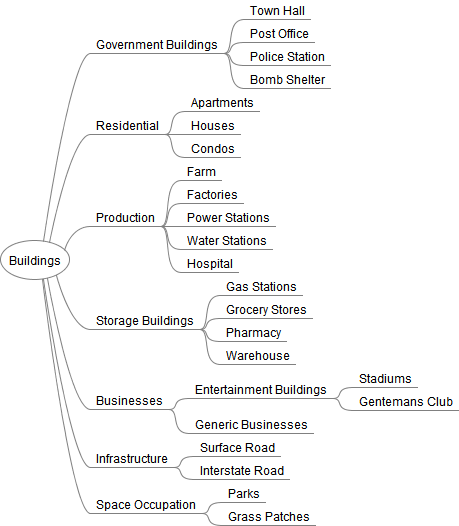
\includegraphics[scale=0.34, trim=4cm 0 4.5cm 0]{../../Diagrams/Buildings/Buildings.png}
  \end{center}

  \end{multicols}

\end{frame}

%-----------END BUILDINGS-----------


\section{Score}

%----------BEGIN SCORE INITIAL----------

\begin{frame}

  \frametitle{Initial Survival Rate}

  \begin{center}
    {\large How many survive the battle?}
  \end{center}

  \begin{outline}
    \1 Each building has a structural integrity rating.
    \1 This rating can be improved by using ``building materials'' on them.
    \1 The likelihood of a building's survival is directly related to its
    structural integrity rating.
    \1 If a building is destroyed, everything inside it is lost - both people and
    resources.
  \end{outline}
  
  \begin{center}
    
\includegraphics[scale=2.0]{../../Images/Apartments.png}
  \end{center}

\end{frame}

%-----------END SCORE INITIAL-----------

%----------BEGIN SCORE PROLONGED----------

\begin{frame}

  \frametitle{Prolonged Survival Rate}

  \begin{center}
    {\large How many survive the war?}
  \end{center}

  \begin{outline}
    \1 How much food is left to feed the survivors?
    \1 How much medical supplies do they have?
    \1 Are there enough resources to farm?
    \1 Is there housing enough for everyone?
  \end{outline}

  \begin{center}
    
\includegraphics[scale=2.0, trim=2cm 0 0 0]{../../Images/grasstile.png}
    
\includegraphics[scale=2.0]{../../Images/grasstile.png}
    
\includegraphics[scale=2.0, trim=0 0 2cm 0]{../../Images/grasstile.png}
  \end{center}
  
\end{frame}

%-----------END SCORE PROLONGED-----------

\section{Implementation}

%----------BEGIN CLASS DIAGRAM----------

\begin{frame}

  \frametitle{Class Diagram}


\end{frame}

%-----------END CLASS DIAGRAM-----------

\section{Demo}

%----------BEGIN DEMO----------

\begin{frame}

  \frametitle{Demo}

  \begin{center}
    
\includegraphics[scale=1.5]{../../Preparation/icon.png}
  \end{center}

\end{frame}

%-----------END DEMO-----------


\end{document}
